\documentclass[11pt]{article}
\usepackage[margin=.92in]{geometry}
\usepackage[T1]{fontenc}
\usepackage[utf8]{inputenc}
\usepackage{lmodern,microtype}
\usepackage{amsmath,amssymb,mathtools}
\usepackage{booktabs,tabularx,array}
\usepackage{graphicx}
\usepackage{enumitem}
\usepackage[dvipsnames]{xcolor}
\usepackage[round,authoryear]{natbib}
\usepackage[colorlinks=true,allcolors=MidnightBlue]{hyperref}
\usepackage[nameinlink,noabbrev]{cleveref}
\usepackage{fancyhdr}
\usepackage{listings}
\usepackage{caption}
\setlength{\headheight}{14pt}
\setlength{\emergencystretch}{2em}
\newcolumntype{Y}{>{\raggedright\arraybackslash}X}
\newcommand{\code}[1]{\texttt{#1}}
\newcommand{\LAPC}{\operatorname{LAPC}}
\definecolor{human}{HTML}{294C60}
\definecolor{machine}{HTML}{B24C3D}
\lstset{basicstyle=\ttfamily\footnotesize,breaklines=true,frame=single,
  xleftmargin=2mm,framexleftmargin=1mm,columns=fullflexible}
\pagestyle{fancy}
\fancyhf{}
\lhead{The horizon of a proof}
\rhead{August 2026}
\cfoot{\thepage}

\title{\textbf{Proofs for Now and Proofs for Later}\\
\large The Amortization Horizon of Human and Artificial Reasoning in Lean}
\author{Working paper}
\date{2 August 2026}

\begin{document}
\maketitle

\begin{abstract}
A checked proof establishes that a proposition follows, but not what future it was built to serve.
We propose the \emph{amortization horizon}: the range over which a
constructor expects an abstraction to repay its cost. A proof consequently has three separable
products---a kernel certificate, external working memory, and an interface for later proofs and readers. We
test this distinction in 3,630 pairs of validated Lean proofs of identical
statements. AI-provenance scripts create more named local claims, but each claim receives fewer
explicit downstream references, crosses fewer later claim boundaries, and is far more often
generically named. A scope-correct analysis of elaborated terms confirms more dead AI binders, yet
finds equal rates of multi-use binders: tactics can turn disposable source state into
kernel sharing. An exploratory Lean-model analysis finds a short information pulse at human claim
boundaries, strongly attenuated at AI boundaries. These results locate the divergence not in deductive power
or biological kind, but in which consumer the construction serves. Recent machine refactoring and
library-building systems support the corresponding prediction: changing the horizon changes the
artifact. We formalize the idea as library-amortized proof complexity over theorem streams, a quantity that
single-theorem benchmarks cannot observe.
\end{abstract}

\section{The missing future of a checked proof}

A theorem prover settles a sharply posed question: did this term check at this type?  That question
is essential, but it is not the whole function of proof.  A mathematician also uses a proof to find
the invariant that makes a result intelligible, to remember a route through an argument, to expose
a lemma that will solve the next theorem, and to leave an object another person can repair
\citep{rav1999}.  These
uses extend beyond the instant of verification.  Two certificates of the same statement may thus
agree perfectly as kernel inputs while serving different futures.

This paper argues that this future is the most useful level at which to compare present human- and
AI-provenance Lean proofs.  The common contrast---human proof versus machine proof---encourages an
essentialist question: what signature does the identity of the constructor leave in a proof graph?
That question is poorly controlled.  Theorem, library, tactic, model, and representation all change
graph statistics.  More importantly, it mistakes an objective for an organism.  Most generated
proofs are rewarded when the current declaration compiles.  Much human formalization occurs inside
a longer activity of exposition, maintenance, and library construction; early workflow evidence
also finds that users want AI assistance while preserving high-level control \citep{collins2026}.
Different artifacts are
therefore rational even before any difference in cognitive machinery is posited.

We call the relevant variable the \emph{amortization horizon}: how far into future reasoning the
constructor expects a present abstraction to pay.  At a short horizon, a local claim can be useful
merely because it records a search result for the next tactic.  Its name need only be distinct; its
statement need not be reusable; it may disappear under elaboration.  At a long horizon, names,
boundaries, generality, and stable dependencies become investments.  Their up-front cost can be
recovered across later steps, theorems, versions, and readers.

This account makes four contributions.  First, it separates three products of formal construction:
certificate, episode structure, and interface.  Second, it tests their separation in 3,630 exact-
statement human--AI pairs, with a scope-aware kernel-term validation on 298 pairs.  Third, it offers
an exploratory information-theoretic test inspired by work on how speakers regulate surprise in
conversation \citep{bergey2024}.  Finally, it proposes a sequence-level object, amortized proof
complexity, that charges for a library and the stream of proofs it enables.  This reframes a central
evaluation problem: success at one theorem measures certificate production, not mathematical
accumulation.

The argument deliberately narrows several earlier claims in this repository.  Viteri and DeDeo's
proof-network work establishes that proof organization can support robust belief and reveals
heavy-tailed reuse \citep{viteri2022}.  Our replication found those results informative but highly
sensitive to the graph boundary.  Near-saturated belief did not distinguish paired certificates,
and a newly discovered de Bruijn-scope conflation makes the inherited unexpanded-term topology
unsuitable as a semantic reuse measure.  Rather than force authorship into those statistics, we use
the failure to identify the missing object: who or what must use the proof next?

\section{A proof has three consumers}

The word ``proof'' compresses at least three artifacts.

\paragraph{Certificate.} The kernel consumes an elaborated term and checks that it inhabits the
target type.  The certificate may contain local \code{let} binders and shared subexpressions, but
the kernel does not require human-readable names, explanatory order, or a useful public API.

\paragraph{Episode structure.} The constructor and an immediate reader consume the source script
during the current attempt.  A named \code{have} makes a fact addressable, reduces the active goal,
and records search state.  It can perform this role even if no later source token names it: a
contextual tactic such as \code{linarith} may consume it implicitly, or elaboration may erase it.

\paragraph{Interface.} Future proofs and maintainers consume exported declarations, stable names,
general statements, and explanatory boundaries.  An interface is not just a set of dependencies.
It is a retrieval scheme: it partitions a derivation into units that can be recognized and invoked
without reconstructing their interiors.  DeDeo and Duede call attention to the associated
correspondence problem: a formal derivation can exist while failing to track the proof idea that is
supposed to justify its relevance \citep{dedeo2026correspondence}.
The interface can also certify something about its constructor: explanatory choices provide
evidence of understanding that bare correctness does not.  Cheap generation can sever this
costly-signal function even while improving verification \citep{wojtowicz2025}.  For this
meta-consumer, construction cost is not mere overhead but part of the evidence; automation may
preserve the visible artifact while changing what its production warrants.

These consumers define different notions of reuse.  A proof-term binder used twice is a sharing
node in a directed acyclic graph.  A source claim referenced after several later claims is working
memory with temporal reach.  An exported theorem cited by later files is persistent memory.  None
is a universal measure of modularity.  In particular, raw occurrence counts can mistake tactic
expansion for conceptual importance, while a theorem that is used only once may still identify the
right explanatory cut.

Elaboration can be viewed as a channel from visible episode structure to the certificate.  A source
boundary can be dependency-deleted (zero term occurrences), transmitted as one compositional hand-off, or
amplified by tactic expansion (multiple occurrences).  Deletion and amplification are not defects,
but both move the certificate away from one-to-one transmission.  We call their combined mass
\emph{certificate polarization}; it measures alignment between episode structure and certificate,
not mathematical quality by itself.

For an abstraction $z$ and consumer $c$, a minimal decision model is
\begin{equation}
 V_{\gamma,c}(z)=\sum_{u\in U_c(z)}\gamma^{d(z,u)}s_c(u)
 -c_{\rm make}(z)-c_{{\rm interface},c}(z),
 \label{eq:value}
\end{equation}
where $U_c(z)$ is the set of anticipated uses, $s_c(u)$ is work saved at use $u$, and $d$ is distance in
steps, theorems, time, or agents.  The discount $\gamma$ summarizes the construction horizon.
Interface work includes choosing a statement at the right generality, selecting a memorable name,
documenting it, controlling imports, and maintaining it across versions.  These costs can dominate
when the only scored outcome is today's compilation.  A short-horizon system may therefore be
globally wasteful while locally optimal.

The consumer index matters as much as the discount.  The same lemma can have positive value for a
retrieval-equipped prover and negative value for a reader who cannot recognize or trust it.  There
is consequently no consumer-free scalar called ``lemma quality.''  Horizon specifies when value
must be recovered; audience specifies whose future work counts.

The principle yields discriminating predictions.  Holding the theorem fixed, a shorter horizon
should produce more local claims that are unused or single-use, less semantic investment in names,
and shorter visible spans between definition and last reference.  It does \emph{not} predict that
every machine claim is unreused, nor that every human claim is explanatory.  Most importantly, it
predicts an intervention: an AI given downstream library and maintenance objectives should cross
the observed divide.  Recent systems that explicitly extract reusable theorems or refactor
generated proofs provide early evidence for exactly this mobility \citep{zhou2024,fu2026refactor,
lu2026leanrefactor,lyu2026rtl2lean}.

\section{Paired observation at three resolutions}

\subsection{Corpus and estimand}

We use the local NuminaMath-LEAN proof-artifact shards \citep{numinamathlean}.  A record is retained when human and prover
proofs are both available and marked valid, the human ground-truth annotation is complete, and the
UUID is unique.  We then require both serialized artifacts to contain the same normalized final
declaration signature.  This audit removes one nominally valid prover artifact with no target and
four mismatches: one wrong theorem join, one helper-only output, and two altered propositions.  The
result is 3,630 exact-statement pairs from 12 coarse source groups.  We analyze only the final target
declaration.  In 158 pairs, both tracks contain identical pre-target declarations after whitespace
and comment normalization; 11 additional AI artifacts introduce helpers named only
\code{lemma\_1} or \code{lemma\_2}, seven of which the target cites.  Pooling these
declarations would therefore mix shared problem scaffolding and side-specific output with the
target-proof comparison, not reveal a human-only miniature library.

The dataset card defines its formal ground truth as a proof written by a human annotator and its
prover field as a model proof produced during reinforcement-learning training \citep{numinamathlean}.
``Human'' and ``AI'' below denote those artifact fields.  This does
not mean unaided human cognition versus an isolated model.  Selection, shared libraries, model
training data, and annotation workflows remain possible causes.  Pairing removes theorem identity,
not those process differences.  Our estimand is consequently descriptive: how these two artifact
tracks differ under the workflows that produced them.

At source level, a Unicode-aware parser removes comments and strings, locates named \code{have}
claims in the final proof body, and counts later exact-name references.  The counting window stops
at same-name redeclaration, a conservative guard against shadowing.  A claim has \emph{long visible
reach} when its last reference occurs after at least one intervening claim boundary.  Names matching
generic forms such as \code{h}, \code{h7}, \code{this}, \code{step2}, and \code{aux} are classified
as placeholders.  Results are pooled at claim level, with 95\% intervals from resampling the 12
source groups.  Pairwise proof metrics use Wilcoxon signed-rank tests; the effect sizes, source
consistency, and sensitivity checks matter more than the very small $p$-values.

Lexical reference is not semantic use.  To validate it we elaborate a preselected 312-pair sample
against current Lean/Mathlib 4.33.0-rc1 and inspect each \code{letE} in the final theorem's proof term.
The dataset was originally checked against Mathlib 4.15.0, so compilation failure under the later
snapshot measures version attrition rather than invalidity at production time.  A
de-Bruijn-aware traversal counts occurrences of a binder while increasing depth under nested
binders; source claims are aligned to term binders by exact-name longest common subsequence in
preorder.  Of 624 tasks, 604 compile; 298 pairs have both sides.  The alignment recovers 3,215 of
3,227 source claims in successful tasks (99.6\%).  A unique-name sensitivity gives the same
direction.  The 20 failures reflect toolchain drift and are reported, not silently replaced.

Finally, we score the 624 source documents in the preselected sample with a local \code{Q4\_K\_M}
quantization of Goedel-Prover-V2-8B \citep{lin2025goedel}.  Each token receives negative log
probability given up to 8,192 preceding tokens.  At each \code{have} boundary we compare the next
4, 8, 16, or 32 tokens with the preceding window and with eligible non-boundary locations in the
same document.  This is model-relative surprise under a prover trained on Lean-like text, not a
measurement of human cognitive surprisal.  Training overlap and affinity for the prover track are
unexcluded.  We therefore treat it as an exploratory timing assay rather than evidence of
understanding.

\subsection{Local claims have different fates}

The paired proofs are not radically different in raw size: median final-body length is 125
whitespace tokens for the human track and 145 for AI, with a median within-pair increase of five
tokens (source-cluster interval 2--15).  They decompose that work differently.  The median number
of named claims is one versus four; pooled density is 1.97 human and 3.17 AI claims per 100 source
tokens.

The important contrast is what happens after introduction (\cref{fig:functions}).  Human claims
receive 1.42 explicit references on average (source-cluster interval 1.32--1.56), compared with
0.86 for AI (0.83--0.88).  Of human claims, 22.9\% have zero visible uptake and 25.7\% have multiple
references.  For AI the corresponding values are 36.4\% and 12.0\%.  All 12 source groups show
lower references per AI claim and higher zero-uptake share.  Human claims also more often remain
live across a later claim boundary: 47.5\% versus 41.7\%, in the human direction for 11 of 12
groups.  The result is not simply that AI proofs are longer; it concerns the conditional fate of an
introduced abstraction.
Nor is it arithmetic from emitting more claims.  In 211 pairs with the same positive claim count,
explicit uses per claim remain 1.36 versus 1.08 (AI-minus-human source-cluster interval
$-0.446$ to $-0.177$), and zero uptake remains 22.4\% versus 29.5\% ($0.047$ to $0.094$).
Nor does repeated generic naming create the result: among names declared only once per proof,
uses are 1.51 versus 0.91, zero uptake 19.9\% versus 33.3\%, and long reach 51.4\% versus 45.9\%.

\begin{figure}[t]
  \centering
  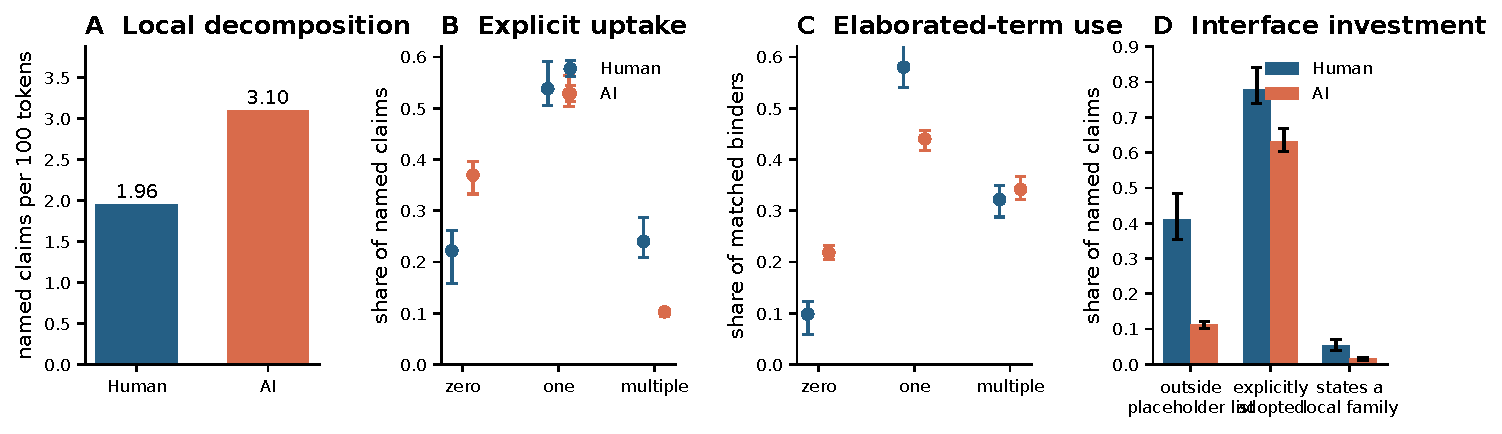
\includegraphics[width=\textwidth]{figures/claim_functions.pdf}
  \caption{Three consumers of local claims. Source results use all 3,630 theorem pairs; term results
  use the 298 pairs that compiled on both sides. Error bars in panels B--D are 95\% source-cluster intervals.
  ``Outside placeholder'' means a name outside the conservative generic-form list; ``long reach'' means the
  last explicit reference crosses at least one later claim boundary.}
  \label{fig:functions}
\end{figure}

Names show an even larger difference.  Placeholder forms account for 58.9\% of human claims and
88.9\% of AI claims.  The pooled human name distribution has 3,522 types, Shannon entropy 8.49 bits,
and effective vocabulary 360; the AI distribution has 1,685 types, 6.27 bits, and effective
vocabulary 77 despite containing 75\% more name tokens.  Length is a crude but convergent check:
23.3\% of human names and 9.4\% of AI names have at least four characters.  This is consistent with
interface investment, but it is not by itself proof of semantic quality.  A short conventional name
may be excellent, and a long name may be decorative.

The elaborated term analysis both confirms and corrects the source story.  Among aligned binders,
14.0\% of human versus 23.4\% of AI claims have zero occurrence in the final theorem term.  Thus the
AI track more often externalizes transient state on which the certificate does not depend.  But the
rate of multiple term occurrences is essentially equal: 35.0\% human and 35.9\% AI.  This is a
substantive falsification of the simplest ``AI does not reuse'' narrative.  Contextual tactics can
duplicate an available fact many times during elaboration; raw mean use counts have enormous
outliers and are not cognitively interpretable.  What survives is more precise: AI introduces more
disposable source state, while kernel sharing among retained binders is not uniquely human.

\begin{figure}[t]
  \centering
  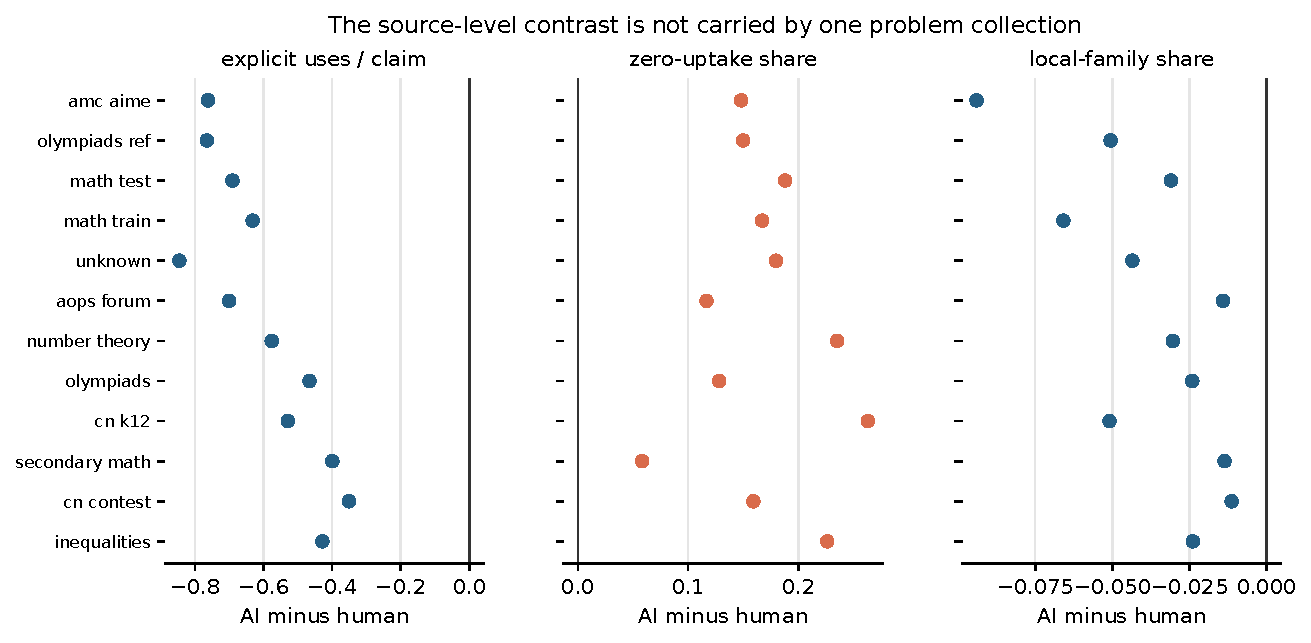
\includegraphics[width=.94\textwidth]{figures/source_consistency.pdf}
  \caption{Source-group consistency. Each point is one of 12 source groups and shows AI minus human.
  References per claim are lower for AI in every group; zero-uptake is higher in every group; long
  visible reach is lower in 11 of 12. Point sizes encode paired sample count.}
  \label{fig:sources}
\end{figure}

\subsection{One theorem, two temporal organizations}

An illustrative pair makes the aggregate distinction legible.  The theorem asks Lean to infer
$x=1$ from
\[
 2^{x^2-2x}+3^{x^2-2x}+x^2-2x+\tfrac16=0.
\]
The human-provenance script names the governing object
$f(t)=2^t+3^t+t$, proves that $f$ is strictly increasing, packages that fact as injectivity, and
uses it to obtain $x^2-2x=-1$.  Its three named claims are \code{e1}, \code{f\_incr}, and
\code{f\_inj}; each is referenced once, and two remain live across a later boundary.

The AI script instead proves the key equality through two cases, below and above $-1$, separately
rederiving bounds for $2^t$ and $3^t$.  It introduces 24 claims named from \code{h1} through
\code{h10}, with names reused in nested scopes.  Eight aligned binders have zero final-term use.
Both proofs check, and both recognize monotonic behavior.  The difference is where that recognition
is stored.  The human version turns it into an addressable invariant; the AI version distributes it
across case-local inequalities.  One creates a small interface inside the proof, the other a trace
of successful search.

This pair was selected because it is clear, not because it is representative by itself.  Reverse
examples exist.  Its evidential role is to interpret the aggregate contrasts, whose paired and
source-stratified directions were fixed independently.

\subsection{Claim boundaries carry a short information pulse}

Human conversational production regulates information in time: pauses and backchannels appear near
changes in information rate \citep{bergey2024}.  If a named claim is an explanatory boundary rather
than only syntax, it might likewise concentrate material that a predictive model finds locally
unexpected.

The exploratory result is compatible with that prediction (\cref{fig:surprise}).  Across the 174
pairs in which both proofs contain eligible boundaries, the median eight-token boundary excess---
post-boundary minus pre-boundary NLL, corrected by same-document control positions---is 0.345 nats
per token for human scripts and 0.024 for AI.  The paired difference is $-0.235$ ($p=3.9\times
10^{-5}$).  Removing the \code{have} keyword and claim name leaves an excess of 0.200 versus 0.042
($p=.021$).  The effect is present in 4- and 8-token windows and disappears by 16 and 32 tokens.
Thus it is a local pulse, not sustained global difficulty.

\begin{figure}[t]
  \centering
  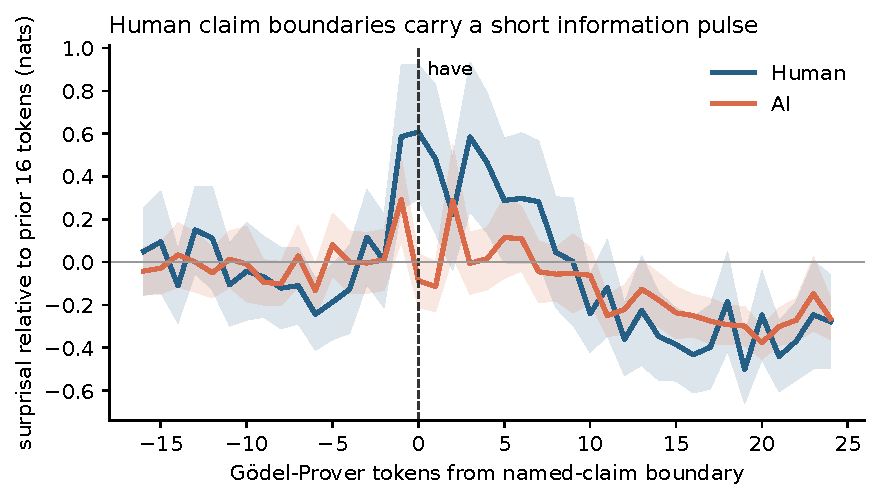
\includegraphics[width=.92\textwidth]{figures/surprise_pulse.pdf}
  \caption{Exploratory model-relative information around source \code{have} boundaries. Curves show
  negative log probability relative to the preceding 16 tokens; bands are proof-weighted 95\%
  standard-error intervals. The model is Goedel-Prover-V2-8B in raw-code mode. The result may
  reflect training overlap, naming conventions, or prover-style affinity and is not a human
  surprisal measurement.}
  \label{fig:surprise}
\end{figure}

The model assigns AI documents much lower NLL overall (median 0.73 versus 1.15), a warning about
style affinity or data overlap.  A leave-one-source-out token bigram preserves the raw boundary
direction ($p=.021$), but its content-only contrast is merely directional ($p=.070$).  We infer
neither creativity nor cognitive surprise.  At most, human boundaries mark a brief predictive
discontinuity whose semantic interpretation remains model-dependent.

\section{From provenance to objective}

The horizon principle would be weak if it merely renamed the observed label.  Its main content is
that the difference should move when the objective moves.  Several recent lines of work support this
prediction.  REFACTOR extracts heavily reused theorems from completed Metamath proofs
\citep{zhou2024}.  Proof-Refactor and Lean Refactor explicitly optimize modularity, maintenance,
checking cost, or version robustness after compilation \citep{fu2026refactor,lu2026leanrefactor}.
CircuitProver provides a closer intervention: accumulating verified lemmas and strategies across
related Lean tasks reduces both proof length and checking time in ablation \citep{yang2026circuit}.
Rtl2lean likewise asks a generator to build a layered reusable library \citep{lyu2026rtl2lean}.

The ingredients have precedents: mined HOL Light inferences, LEGO-Prover, and DreamProver all turn
intermediate results into later proving capacity \citep{kaliszyk2014,wang2023lego,zhang2026dream}.
They also expose the retrieval constraint: persistent memory helps only if a later agent can select
it; LeanSearch v2 reports a large gain from global premise retrieval \citep{gao2026leansearch}.
Our contribution is a common account of compile-first artifacts, refactored proofs, readable
boundaries, and growing libraries, plus an objective that charges construction against future savings.

These systems do not prove that their artifacts match mature human libraries, and their metrics are
not directly comparable with ours.  They establish the more fundamental point: machines can be
made to externalize persistent mathematical memory.  The observed human--AI difference is therefore
best read as a difference between present production regimes.  The causal experiment now suggested
is straightforward: assign the same base model the same theorem stream under (i) per-theorem compile
reward and (ii) downstream cost, maintenance, and human-retrieval reward.  Measure dead binders,
claim reach, API survival, later citation, repair cost, and reader comprehension.  If the horizons
do not separate, our account fails.

The distinction also clarifies DeDeo's discussion of ``alien lemmas.''  His argument draws on
proof-complexity and average-case results to contrast hard-to-prove truths with a mathematical
practice that seems to select truths with good reasons \citep{dedeo2024hard}.  An AI may discover a lemma that dramatically
compresses later certificates yet remains unrecognizable to human mathematical ontology.  Such a
lemma has high machine amortized value and low human interface value.  It is neither simply good nor
bad.  It exposes two horizons with different consumers.  The correspondence problem then becomes an
engineering and epistemic demand: construct a bridge that preserves the machine compression while
letting human readers track why the abstraction matters \citep{dedeo2023aleph,
dedeo2026correspondence}.

\section{Cognitive implications: abstraction as memory allocation}

The source-level difference suggests a cognitive interpretation more specific than ``humans are
abstract'' and more defensible than reading mental states directly from code.  Constructing a proof
requires allocating limited representational capacity.  A solver can preserve the past by keeping
facts in the local context, by naming a relation that summarizes many facts, or by retrieving a
library theorem that packages an older derivation.  These are memory operations at different
scales.  The horizon determines which compression is worth performing.

At the scale of one search episode, an intermediate claim can function like a checkpoint.  It
freezes a successful subcomputation, constrains the remaining goal, and provides the next tactic
with an enlarged context.  Generic labels are adequate because identity can be recovered from
position.  Dead elaborated binders are not necessarily mistakes on this account.  They are traces
of a search process whose utility was exhausted before the final certificate.  Removing them may
improve the artifact while making the original generation harder to understand, just as deleting a
scratch calculation produces a cleaner solution but erases evidence about discovery.

At a longer scale, an abstraction is a lossy compression chosen for transfer.  The statement
forgets derivational detail while preserving a relation expected to matter again.  A descriptive
name supplies a retrieval cue; a proof boundary asserts that the interior can be temporarily
ignored; a general signature enlarges the class of future contexts in which the package applies.
This compression is not free.  Choosing the wrong invariant can increase working-memory demand,
and exporting too many lemmas makes the library harder to search.  Long-horizon construction is
therefore not maximization of lemma count.  It is selection of a small basis whose elements remain
useful after the local context has vanished.

The equality of multi-use term binders is theoretically important here.  Kernel sharing and
communicative abstraction are different achievements.  Automation can expand a generic hypothesis
into many term occurrences without ever identifying a concept for a reader.  Conversely, a
well-chosen explanatory lemma can deserve a name even when invoked once in the current theorem,
because its intended reuse lies in another proof or another mind.  Any cognitive account based
only on the certificate DAG will confuse these cases.  The units of human mathematical thought are
not guaranteed to coincide with the compiler's units of common-subexpression elimination.

The local surprisal pulse offers a tentative temporal signature of this selection.  A useful
boundary often arrives when prior manipulations have made a new description possible: monotonicity,
invariance, symmetry, or a change of representation.  The words immediately after the boundary can
therefore be hard to predict from nearby syntax even though the resulting claim makes the rest of
the argument easier.  In conversational terms, the constructor briefly spends information to
renegotiate common ground.  The pulse's disappearance after 16 tokens is consistent with a boundary
event rather than generally ornate prose.  But this interpretation must remain provisional until
human reading time, recall, and transfer are measured directly.

This perspective also distinguishes discovery from presentation without separating them
absolutely.  A source proof can be a search trace, a pedagogical artifact, or both.  Humans often
refactor scratch work into a proof idea; present generators are commonly evaluated before that
second pass.  The central divergence may thus be procedural: one workflow includes consolidation,
naming, and anticipation of reuse, while another terminates at verification.  A cognitively serious
comparison should align stages---first attempts with first attempts, refactored artifacts with
refactored artifacts---and observe how representations change between them.  The horizon principle
predicts that the largest human--AI gap will occur not in local inference, where both can exploit
formal context, but in deciding what part of a successful episode should become shared memory.

\section{Library-amortized proof complexity}

Ordinary proof complexity asks for the size of a certificate for one formula in a fixed proof
system \citep{cook1979,krajicek1995}.  This leaves library construction outside the objective.  Let
$\Phi=(\varphi_1,\ldots,\varphi_T)$ be a stream of targets.  Let $L$ be an ordered, acyclic sequence
of auxiliary declarations: each signature and body must check in the base environment plus earlier
members of $L$, and $|L|$ charges both.  If $P_t$ checks $\varphi_t$ in that extended environment and
$|P_t\mid L|$ is its residual certificate size, define
\begin{equation}
 \LAPC_\lambda(\Phi)=
 \min_{L,P_1,\ldots,P_T}
 \left[\lambda |L|+\sum_{t=1}^T |P_t\mid L|\right],
 \label{eq:apc}
\end{equation}
with $\lambda\geq 1$.  Thus neither a circular declaration nor an unpriced advice oracle is allowed.
The factor $\lambda$ prices the design and maintenance of shared structure.  A richer version can price names,
dependency fragility, retrieval, and human validation separately.  An online version charges when
each declaration is introduced and compares cumulative cost with the best hindsight library.

Let $C(\varphi)$ be the shortest proof of one target without a new library.  Because $L$ may be
empty, $\LAPC_\lambda(\Phi)\leq\sum_t C(\varphi_t)$.  The gap
\begin{equation}
 G_\lambda(\Phi)=\sum_t C(\varphi_t)-\LAPC_\lambda(\Phi)
 \label{eq:gain}
\end{equation}
is the compression attributable to shared mathematical infrastructure at the chosen interface
price.  At $\lambda=1$ the objective is a restricted two-part description length: library plus
residual certificates.  It is not Kolmogorov complexity; the language is fixed to checked Lean
artifacts and retrieval cost can be charged explicitly.

The break-even law is immediate but useful.  Ignoring interactions, a declaration of charged size
$b$ that saves $s$ symbols in each of $k$ residual proofs pays exactly when $ks>\lambda b$; with
temporal discounting, $ks$ becomes $\sum_i\gamma^{d_i}s_i$.  The amortization horizon is therefore
not a metaphor but the point at which checked shared structure beats repeated local construction.

Equation \eqref{eq:apc} changes what counts as an optimal proof.  A declaration that lengthens the
first episode may lower total cost if it compresses later proofs.  A generic helper that is short
but impossible to retrieve may fail to pay back its interface cost.  A benchmark of independent
theorems with a reset context implicitly sets future reuse to zero and selects a compile-first
policy.  Even pass@$k$ with enormous search budgets remains a measure of finding current
certificates, not of learning a mathematical language in which later certificates become cheap.

The connection to circuit sharing and extension variables is instructive but limited.  Naming a
repeated subexpression turns tree accounting into DAG accounting; introducing a reusable theorem
resembles adding a subroutine or grammar rule.  Yet Lean claims are dependent types, tactics alter
elaboration, definitions compute, and public theorem statements carry semantic and maintenance
costs.  We do not claim an equivalence with Extended Frege.  The robust lesson is accounting level:
single-certificate complexity cannot see investments whose return lies across certificates.

This produces new empirical questions at the boundary of complexity and cognition.  How large can
online library regret be for a bounded-context agent?  Which theorem orderings permit discovery of
the hindsight-optimal abstractions?  Does a human-readable interface impose only polynomial overhead
on a machine-efficient lemma basis, or can correspondence itself be exponentially costly?  DeDeo's
``hard proofs'' dilemma suggests that mathematical culture may be understood as a selection process
over theorem streams and representations, concentrating attention where useful proofs and reasons
coincide \citep{dedeo2024hard}.  AI changes both the search distribution and the consumers for whom
that coincidence must hold.

\section{What the result does and does not establish}

The evidence supports a narrow, structural claim.  In this paired corpus, the AI track uses more
source-level local state; more of it is visibly unreferenced, more of it vanishes from the final
term's dependency structure, its names are more generic, and its visible temporal reach is shorter.
It does not support a claim that machine proof terms lack sharing: retained binders are multiply
used at the same rate.
Nor does it show that human artifacts are globally reusable, since our primary analysis ends at the
target declaration.  The distinction between episode and persistent interface remains to be tested
on theorem sequences.

Several limitations are consequential.  First, source provenance is observational.  Second, the
lexical parser recognizes named \code{have}, not every \code{let}, \code{suffices}, anonymous claim,
or tactic-generated subgoal.  Third, compilation leaves 298 complete pairs in the term sample;
although their source patterns resemble the full corpus, toolchain attrition can select on style.
Fourth, binder occurrence is syntactic and can be amplified massively by automation.  Fifth, the
main surprisal model may have seen related text, while a source-held-out bigram weakens the
content-only contrast.  The boundary effect is exploratory.  Sixth, meaningful names and long spans are only proxies
for explanatory value.  Interactive links from written proof steps to Lean state have improved
comprehension in a small reader study, but our boundary measures still require a direct experiment
\citep{kambhamettu2026}.

The representation audit adds one correction.  An earlier root-term extractor globally interned
raw de Bruijn indices from unrelated scopes, creating false reuse paths.  Scope-specific identities
remove the error, and a corrected 298-pair rerun finds no robust authorship effect in either the
fixed-$10$ reuse-tail exponent ($-0.002$, source-cluster interval $-0.016$ to $0.013$) or maximum
outdegree (median difference zero, $-3$ to $0$).  The binder-use traversal here is independently
scope-aware; details and regression construction appear in the appendix.

Three observations would falsify or sharply narrow the horizon account.  The claim fails if an
objective-matched human--AI experiment retains the same difference; if downstream reward does not
produce longer-lived machine interfaces; or if the proposed interface measures fail to predict
future proof cost, maintenance, or reader comprehension.  Conversely, a machine system that builds
a durable, intelligible library is not an exception to be explained away.  It is the decisive
prediction.

\subsection{Three decisive experiments}

The first experiment is a horizon swap.  Give humans and machines the same ordered Lean tasks and
the same base library.  In one condition, discard each proof after checking it.  In the other, make
every later task cheaper when an earlier abstraction is reusable and charge for broken or
unretrievable APIs.  The critical statistic is the interaction between constructor and condition.
A stable provenance effect would contradict the objective-level account; convergence within
condition would support it.

The second is a consumer swap.  Hold certificates fixed and ask three consumers to operate on
alternative refactorings: the kernel, a new prover with bounded context, and a human reader.  Kernel
cost measures certificate function; downstream search measures machine interface value; delayed
recall, error localization, and transfer measure human interface value.  This design can reveal
alien lemmas rather than assuming them: an abstraction has high value for one consumer and low
value for another.  A correspondence layer succeeds when it raises human value without destroying
machine savings.

The third is a longitudinal library experiment.  Allow an agent to choose which intermediate facts
to export before seeing future targets; measure cumulative cost and survival across orderings and
Lean versions; and compare online choices with a hindsight refactoring.  A system that proves every
target but accumulates high regret has mastered deduction without allocating durable mathematical memory.

These experiments replace artifact classification with a causal question: which incentives transform
successful reasoning into capacity that survives a change of context, consumer, or time?

\section{Conclusion: a proof is a wager on its next use}

A checked certificate has no intrinsic audience beyond the kernel.  Proof construction becomes
mathematical practice when it anticipates another consumer: a later step, a future theorem, a
maintainer, a reader, or another agent.  Human- and AI-provenance Lean proofs of the same statement
currently diverge most clearly here: one track more often packages named, longer-lived hand-offs;
the other records more disposable local state.  After elaboration both can exhibit extensive
sharing.  The difference is not validity or biological kind, but the future for which construction
was optimized.

Proof quality is therefore an amortization question: who will use this boundary, over what distance,
and what work will it save?  A sequence of isolated successes can grow without becoming a library.
Evaluation should ask whether proving today changes tomorrow's cost and intelligibility.

\clearpage
\bibliographystyle{plainnat}
\bibliography{references}

\appendix
\clearpage
\section{Reproducibility and robustness}

All reported paired source results are produced by \code{code/paired\_horizon.py}; scope-aware term
use by \code{code/extract\_binder\_use.py} and \code{code/analyze\_binder\_use.py}; and surprisal by
\code{code/prepare\_surprisal.py}, \code{code/token\_surprisal.cpp},
\code{code/ngram\_surprisal.py}, and \code{code/analyze\_surprisal.py}.  Machine-readable summaries live in \code{results/horizon/}.
Seeds and inclusion rules are serialized with the estimates.

Source intervals resample 12 source groups with replacement and recompute pooled claim ratios.
Every source group has lower explicit uses per AI claim and higher AI zero-uptake; 11 of 12 have
lower AI long-reach share.  The term alignment's unique-name subset contains 753 human and 1,258 AI
claims; zero-use shares are 13.8\% and 23.8\%, respectively.  The surprisal boundary contrast is
present for four- and eight-token windows, marginal at 16, and absent at 32.  Excluding the keyword
and claim name preserves the four- and eight-token effects.  In the leave-one-source-out bigram,
which excludes every document in the held-out proof's coarse source group from training, the raw
eight-token difference remains ($p=.021$) but content-only evidence weakens ($p=.070$).

The preselected 312-pair term sample closely preserves the source contrasts.  Human/AI claim
densities are 1.96/3.25 per 100 tokens in the sample versus 1.97/3.17 in the full corpus; explicit
uses per claim are 1.35/0.84 versus 1.42/0.86; and zero-uptake shares are 22.9\%/35.7\% versus
22.8\%/36.4\%.  All 12 source groups remain represented.  Compilation attrition reduces this to 298
complete binder-use pairs but changes the profile little.

Paired does not mean independent: 181 structured proof values are token-identical and 230 have
whitespace-token similarity at least .90 after comments and strings are removed.  These pairs
attenuate rather than create the result.  Of the 181 exact value matches, 180 also have identical
source bodies, so they are duplicate mass rather than a source/certificate natural experiment.
Excluding all 230 leaves 3,400 pairs; explicit uses per
claim are 1.42/0.85, zero-uptake shares 22.9\%/36.7\%, and placeholder shares 59.0\%/89.5\%.

The source direction also survives a coarse automation sensitivity.  For each of \code{linarith},
\code{nlinarith}, \code{norm\_num}, \code{omega}, \code{ring}, and \code{simp}, we separately retain
pairs in which both sides invoke the tactic and pairs in which neither does.  Across all 12 strata,
AI claims have fewer explicit references per claim and a higher zero-uptake share.  This does not
equate full tactic workflows, but rules out any one of these common families as a sufficient
explanation.

\section{Why the old network result is not the new result}

The prior project replicated Viteri and DeDeo's fixed-tail power-law results and modeled epistemic
phase transitions across Coq and Lean.  Those are properties of declared network constructions.
They do not supply a representation-invariant authorship signature.  Tail exponents move when the
minimum degree or expansion boundary moves; human--AI directions can reverse under proof-value
normalization; and modeled theorem belief is close to saturation in both tracks.

The scope audit strengthens the reason for restraint.  A de Bruijn index identifies a binder by
distance in its local expression, not by a global name.  Interning equal raw indices across scopes
turns distinct variables into one graph node.  The corrected traversal carries a scope environment
and replaces each entered binder with a fresh free-variable identity before hashing expressions.
The regression proof has two independent identity lambdas; the old representation produces one
shared variable leaf, while the corrected representation produces two.  None of the main analyses
in this paper uses a raw-term reuse tail.

The scope-correct rerun elaborates 302 of 312 tasks on each side; applying the independent binder-
task status filter leaves 298 complete pairs.  AI terms are slightly larger (median paired node
difference 88.5; source-cluster interval 0--243) and have a slightly larger visit-to-unique-node
ratio (difference 0.0068; 0.0023--0.0112).  But the proposed authorship signal in high-outdegree reuse remains absent:
maximum outdegree and the fixed-$10$ tail exponent have intervals crossing zero.  These graph
quantities remain representation-specific diagnostics, not measures of cognitive abstraction.

\section{A proposed causal benchmark}

A strong test would sample theorem sequences, not independent goals.  Randomize capable agents to a
compile-first condition or a library condition.  Both receive the same base library, target order,
Lean version, and inference budget.  The library condition is charged for current proof cost but
rewarded for reductions in later search, version repair, and blinded reader retrieval.  Public
declarations must be generated before future targets are revealed to prevent hindsight leakage.

Primary outcomes should include cumulative checked-token or search cost, online regret against a
hindsight refactoring, survival of generated APIs under version changes, cross-target citations,
dead local binders, and delayed human comprehension.  A swap condition---humans under disposable
single-goal incentives and AI under persistent-library incentives---would separate constructor from
horizon.  The strongest result for the present theory would be a crossover interaction rather than
a persistent main effect of provenance.

\end{document}
